\chapter{実装の方針} \label{implementation}

フロントエンドに lively.next~\cite{ingalls_2008} を、方程式の処理と数値計算に SymPy~\cite{meurer_sympy_2017} を用い、JavaScript で実装する。lively.next は、GUIアプリケーションを作成・実行するためのWebプログラミング環境である。学習者が物体や方程式を定義する画面とシミュレーションを表示する画面を lively.next で作成する。SymPy は、記号計算のための Python ライブラリであり、Pyodide~\footnote{\tiny{\url{https://github.com/pyodide/pyodide}}} を用いることで WebAssembly に変換し、ブラウザで実行する。\simname は、入力された物理量や方程式を SymPy オブジェクトに変換することで、数値計算を可能にする。シミュレーションの実行時は、設定された時刻 $t$ の範囲を粒度 $\Delta t$ ずつ変化させる。各方程式に各 $t$ を代入した結果を lively.next が受け取り、描画する。シミュレーションのリアルタイム性を確保するため、各 $t$ を方程式に代入した値は方程式の定義時・変数の値の変更時にあらかじめ計算する。


% 実装は、フロントエンドに lively.next\footnote{\url{https://lively-next.org}} を、文字式の計算に SymPy\footnote{\url{https://www.sympy.org/en/index.html}} を用いた。SymPy は Python のライブラリであるが、WebAssembly で実装された CPython 処理系の Pyodide\footnote{\url{https://pyodide.org/en/stable/}} を用いることでブラウザ上で完結させた。また、数式の表示には KaTeX\footnote{\url{https://katex.org}} を用いた。

% \section{lively.next}
% lively.next は、Lively プロジェクト\footnote{\url{https://www.lively-kernel.org/index.html}}の一つで、ブラウザ上でプログラミングができる環境である。シミュレーション画面とそれぞれの値、SymPy を用いた計算用の画面を lively.next 上で実装している。

% \section{SymPy}
% SymPy は、文字式の計算を可能にするPythonライブラリである。図\ref{SymPy_example}に簡単な例を載せる。SymPyを用いることで、実際に物理の問題を解くように文字式の計算を実行することができる。数値の代入も可能なため、シミュレーションを実行する際は SymPy で表現された式に数値を代入して計算している。

% \clearpage
% \begin{figure}
% 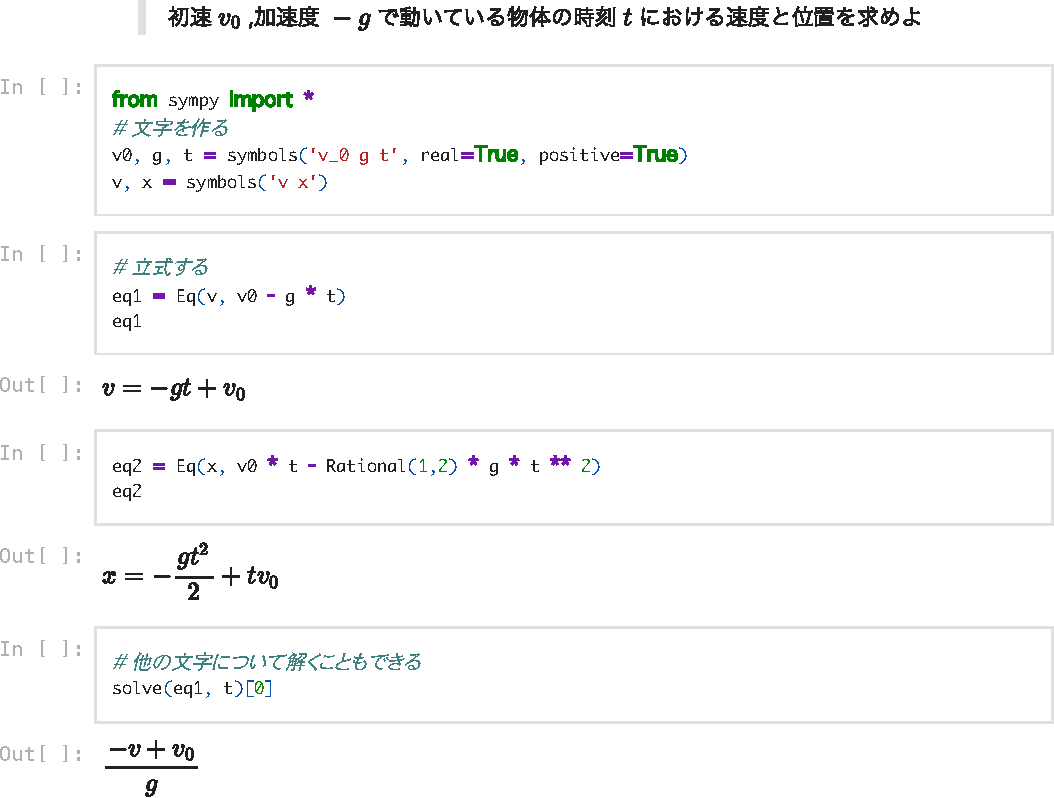
\includegraphics[page=1, scale=.8]{work/SymPy_example-crop.pdf}
% \caption{SymPyを用いた文字式の計算例} \label{SymPy_example}
% \end{figure}
% \clearpage

% \section{Pyodide}
% Pyodide は、Mozilla が開発している WebAssembly で実装された CPython 処理系である。ブラウザ上で Python コードを実行できるほか、メジャーなパッケージにも対応している。 SymPy も Pyodide で実行可能である。実際に Pyodide で SymPy を実行する計算の例を図\ref{Pyodide_example}に、結果を KaTeX を用いて表示した例を図\ref{Pyodide_result}に記す。

% \newgeometry{left=1cm, right=1cm}
% \begin{figure}[htb]
% \begin{lstlisting}[language=html]
% <!DOCTYPE html>
% <head>
%   <script src="https://cdn.jsdelivr.net/pyodide/v0.22.0/full/pyodide.js"></script>
%   <link rel="stylesheet" href="https://cdn.jsdelivr.net/npm/katex@0.16.4/dist/katex.min.css" integrity="sha384-vKruj+a13U8yHIkAyGgK1J3ArTLzrFGBbBc0tDp4ad/EyewESeXE/Iv67Aj8gKZ0" crossorigin="anonymous">
%   <script defer src="https://cdn.jsdelivr.net/npm/katex@0.16.4/dist/katex.min.js" integrity="sha384-PwRUT/YqbnEjkZO0zZxNqcxACrXe+j766U2amXcgMg5457rve2Y7I6ZJSm2A0mS4" crossorigin="anonymous"></script>
%   <script defer src="https://cdn.jsdelivr.net/npm/katex@0.16.4/dist/contrib/auto-render.min.js" integrity="sha384-+VBxd3r6XgURycqtZ117nYw44OOcIax56Z4dCRWbxyPt0Koah1uHoK0o4+/RRE05" crossorigin="anonymous" onload="renderMathInElement(document.body);"></script>
% </head>
% <body>
%   <script>
%     async function main() {
%       let pyodide = await loadPyodide();
%       await pyodide.loadPackage("sympy");
%       let code = `
%       from sympy import symbols, Eq, solve, latex
%       v0, g, t = symbols('v_0 g t', real=True, positive=True)
%       v = symbols('v')
%       eq1 = Eq(v, v0 - g * t)
%       latex(solve(eq1, t)[0])
%       `;
%       let result = pyodide.runPython(code);
%       let resultDiv = document.getElementById("result");
%       resultDiv.textContent = `\\[${result}\\]`;
%       renderMathInElement(resultDiv);
%     };
%     main();
%   </script>
%   <p>結果</p><div id="result" style="float: left"></div>
% </body>
% \end{lstlisting}
% \caption{Pyodide を実行する例} \label{Pyodide_example}
% \end{figure}
% \restoregeometry

% \begin{figure}[htb]
% \centering
% 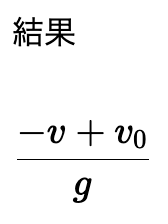
\includegraphics{work/pyodide_screenshot.png}
% \caption{実行結果} \label{Pyodide_result}
% \end{figure}
